\chapter{Methods}


\textit{\textendash\ ``Open the gates now. Private, lower your weapon''. \\ 
\textendash\ ``Not till we feed these people. Court martial me, sir. Do whatever you want with me but not till those people are fed''.\\
\textemdash\ ``Black 47'' by Lance Daly}	

\vspace{.2cm}

\section{Generalized Additive Model}

Due to the difficulty in capturing the non-linear relationship, it is necessary to use scatter plots to observe what the non-linear relationship between the independent and dependent variables is. Figure 4.1 provides an overview of the relationship between independent and dependent variables. The three scatter plots in the first column represent three sets of independent and dependent variables with significant linear relationships, while the three scatter plots in the second column represent three sets of non-significant linear, or non-linear, relationships.

Based on the theory of the entitlement approach mentioned earlier, it is indeed possible that there is a non-linear relationship between the independent and dependent variables, for example, when the price of cereals rises marginally, farmers may grow as a result of this profit, whereas when the price of cereals rises significantly, the farmers' trade-base entitlement is consequently jeopardized, and the population of the year ends up declining. According to this logic, linear regression is not a very good choice here and it is necessary to take other forms of non-linear regression for analysis. 

In the scatter plot of Figure 4.1, a non-linear trend can be observed for all three variables in the second column, for example, for wages, it seems that the initial rise was very beneficial for the farmers' production-based entitlement, and as it continued to rise there was a diminishing marginal benefit in economic theory.

\begin{figure}[h]
    \centering
    \caption{Regression Scatter}
    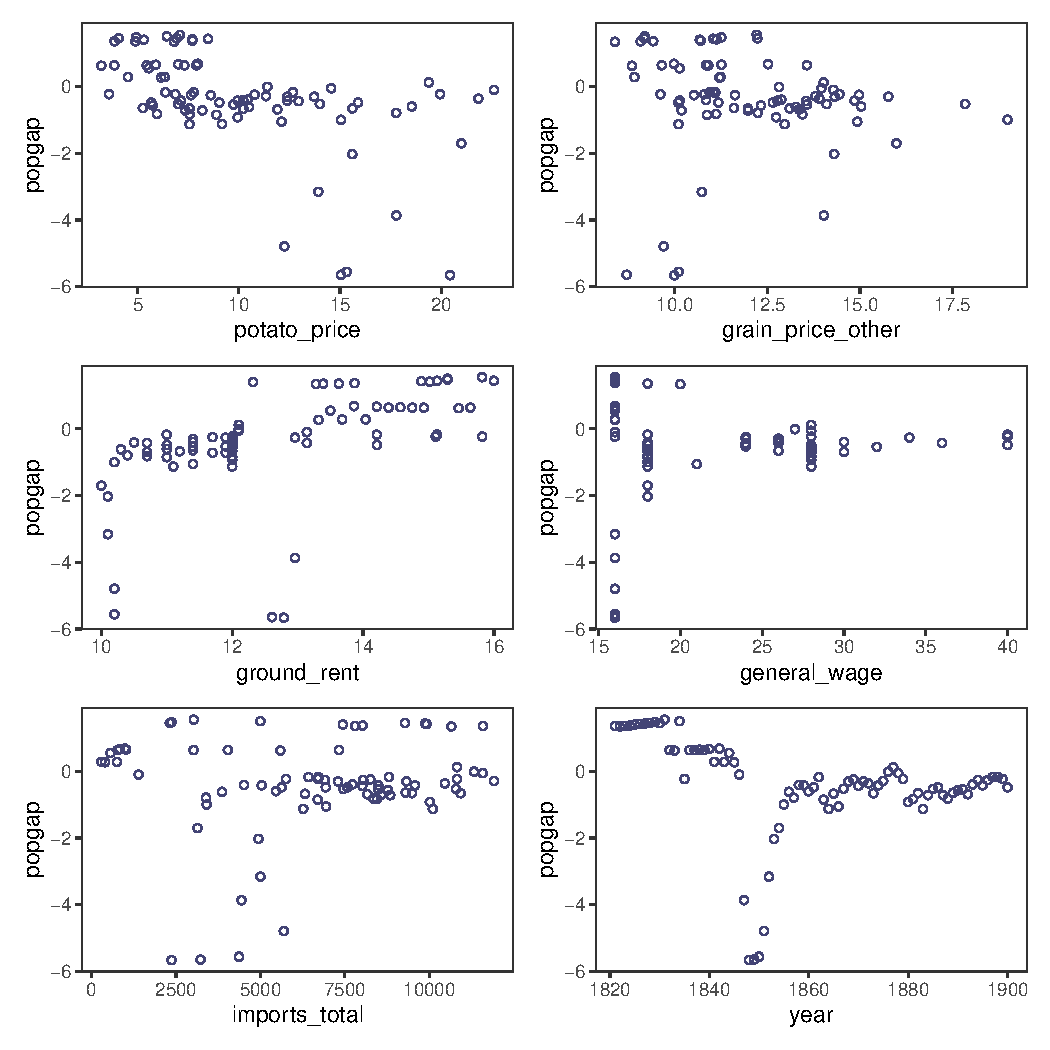
\includegraphics[width=.95\textwidth]{../03_outputs/regression_scatter.pdf}
\end{figure}

Variables in regression included: \texttt{potato\_price}, \texttt{grain\_price\_other}, \texttt{ground\_rent}, \texttt{if\_tithe}, \texttt{general\_wage}, \texttt{poorlaw}, \texttt{imports\_total}, \texttt{exports\_total}. The second regression model includes the variables \texttt{grain\_acre\_total}.

Generalized additive model was used as the main approach in this paper since it is efficient in solving non-linearly relationship from variables by using smooth functions. Based on observation of scatter and correlation matrix, a smoothing function was added to the variables \texttt{grain\_price\_other}, \texttt{general\_wage}, and \texttt{exports\_total}. 

The formulation of the regression model, including the assumptions, is as follows:
\vspace{-14pt}
\begin{align*}
\texttt{E(popgap)} = & \ \beta_0 + \beta_1 \times \texttt{potato\_price} + f_1(\texttt{grain\_price\_other}) \ldots \textit{(H1)} \\
                & + \beta_2 \times \texttt{ground\_rent} + \beta_3 \times \texttt{factor(if\_tithe)} \ldots \ldots .. \textit{(H2)} \\
                & + f_2(\texttt{general\_wage}) \ldots \ldots \ldots \ldots \ldots \ldots \ldots \ldots \ldots \ldots \ldots . \textit{(H3)} \\
                & + \beta_4 \times \texttt{imports\_total} + f_3(\texttt{exports\_total})\\
                & + \beta_6 \times \texttt{factor(poorlaw)} \ldots \ldots \ldots \ldots \ldots \ldots \ldots \ldots \ldots . .. \textit{(H4)} \\
                & + \epsilon
\end{align*}
\vspace{-2cm}
\begin{align*}
\texttt{popgap} = & \ \beta_0 + \beta_1 \times \texttt{grain\_acre\_total}  \ldots \ldots \ldots  \ldots \ldots \ldots \ldots \ldots (\textit{H5a/5b}) \\
& + \epsilon
\end{align*}

This paper fits two regression model. The first regression model is a GAM model, which is used to prove H1, H2, H3 and H4; the second regression model, due to the linear relationship between variables \texttt{grain\_acre\_total} and \texttt{popgap}, is a linear regression, which is used to prove H5. In fact, for the second regression model, the linear regression and the GAM model have the same AIC, and to follow the modeling principle of simplicity, linear regression is used for fitting.

The necessity and feasibility for the use of the GAM model must be justified before proceeding with the regression analysis. Firstly, the VIF test between the variables shows that there is no multicollinearity between the variables (Table 4.1):

\begin{table}[!htbp] \centering 
    \caption{Model Variance Inflation Factors (VIF)} 
    \label{vif_table} 
    \begin{tabular}{lcccc} 
    \\[-1.8ex]\hline 
    \hline \\[-1.8ex] 
    Variable & VIF & Variable & VIF \\ 
    \hline \\[-1.8ex] 
    potato\_price & 2.044 & general\_wage & 5.390 \\ 
    grain\_price\_other & 1.739 & imports\_total & 6.844 \\ 
    ground\_rent & 3.716 & exports\_total & 1.918 \\ 
    factor(if\_tithe)1 & 5.666 & factor(poorlaw)1 & 4.606 \\ 
    \hline 
    \hline \\[-1.8ex] 
    \end{tabular} 
  \end{table}

Compared to linear regression, the GAM was found to have a significantly higher R-squared and a lower AIC, so it can be concluded that the GAM possesses a better fitting ability and explanatory performance. Figure 4.2 shows the details:

\begin{table}[h] 
    \centering 
    \caption{Regression Results: GAM and Linear} 
  \begin{tabular}{@{\extracolsep{5pt}}lcc} 
  \\[-1.8ex]\hline 
  \hline \\[-1.8ex] 
   & \multicolumn{2}{c}{\textit{Dependent variable:}} \\ 
  \cline{2-3} 
  \\[-1.8ex] & \multicolumn{2}{c}{popgap} \\ 
  \hline \\[-1.8ex] 
   & GAM & LM \\ 
  \hline \\[-1.8ex] 
  \multicolumn{3}{c}{Coefficients are omitted to save space and will be shown in next Chapter} \\
  \hline \\[-1.8ex] 
  Observations & 80 & 80 \\ 
  Adjusted R$^{2}$ & 0.741 & 0.570 \\ 
  AIC & 201.470 & 235.916\\
  Residual Std. Error &  & 0.990 (df = 71) \\ 
  F Statistic &  & 14.115$^{***}$ (df = 8; 71) \\ 
  \hline 
  \hline \\[-1.8ex] 
  \textit{Note:}  & \multicolumn{2}{r}{$^{*}$p$<$0.1; $^{**}$p$<$0.05; $^{***}$p$<$0.01} \\ 
  \end{tabular} 
\end{table} 
The model was tested with \texttt{gam.check()} in \texttt{R}, returning results in Figure 4.2.

\begin{figure}[h]
    \centering
    \caption{Regression Check}
    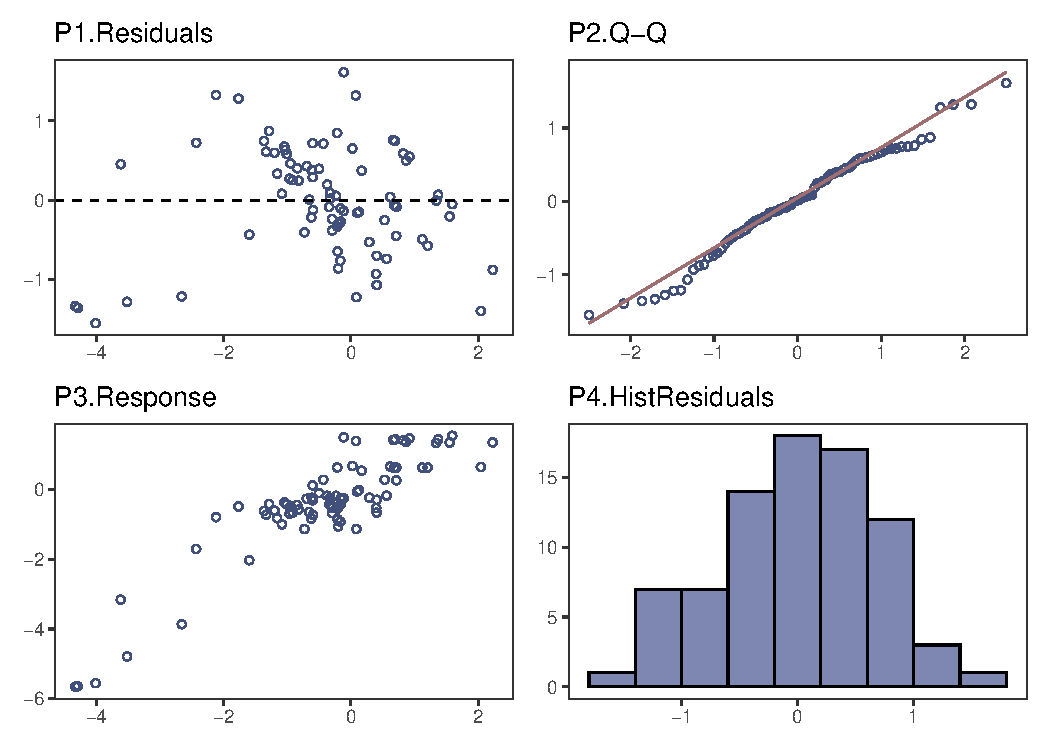
\includegraphics[width=.9\textwidth]{../03_outputs/regcheck.pdf}
\end{figure}
\vspace{-7pt}

From $P1$, it appears that the distribution of the residuals revolves around the $Y=0$ line with a mean approximately equal to 0 and no pattern can be found; whereas the Q-Q plot of $P2$ indicates a normal distribution structure of the data; $P3$ also shows a uniform and random distribution between the response value and fitting value; and finally, the residuals indicated by $P4$ show a normal distribution.

\section{Brief Summary}

An overview of the research logic used throughout the article is given.

First is the theoretical framework: (1) entitlement approach used by Amartya Sen in his book ``Poverty and Famine'', and (2) refutation of the FAD theory. According to Sen's construct, the entitlement approach consists of the following four indicators: trade-based entitlement, production-based entitlement, own-labour entitlement and Inheritance and transfer entitlement; while the FAD theory includes one indicator, the area under food cultivation. This paper generalizes the entitlement approach as a demographic and developmental mechanism based on the literature and attempts to explore if the changes in people's entitlements, which is the independent variable, will affect population change within the year, which is the dependent variable.

Further, hypotheses are made on the basis of these indicators, with each indicator corresponding to a hypothesis and each hypothesis corresponding to a more specific variable in the dataset. $H1$ corresponds to price of potatoes and other cereals, $H2$ corresponds to ground rent and presence or absence of tithing, $H3$ corresponds to general wage, $H4$ corresponds to the imports and exports amount, and the Poor Law, and $H5$ corresponds to the grain planting acreage.

The GAM was used in this study for a number of reasons, including (1) there is no significant linear relationship between some independent variables and the dependent variable, but there is an observable nonlinear relationship and theory supports the existence of such a nonlinear relationship, and (2) the introduction of a smoothing function in the GAM can predict this nonlinear relationship in a good way. Relative tests have been performed before formally discussing the regression, including the VIF test for multicollinearity, AIC and R-square comparisons for linear regression, the residual randomness test, and the residual normality test. All of the results identify the GAM as a reasonable regression model under this data.

Figure 4.3 visualizes the framework of the entire research.

\begin{landscape}
    \begin{figure}[h]
        \centering
        \caption{Research Framework}
        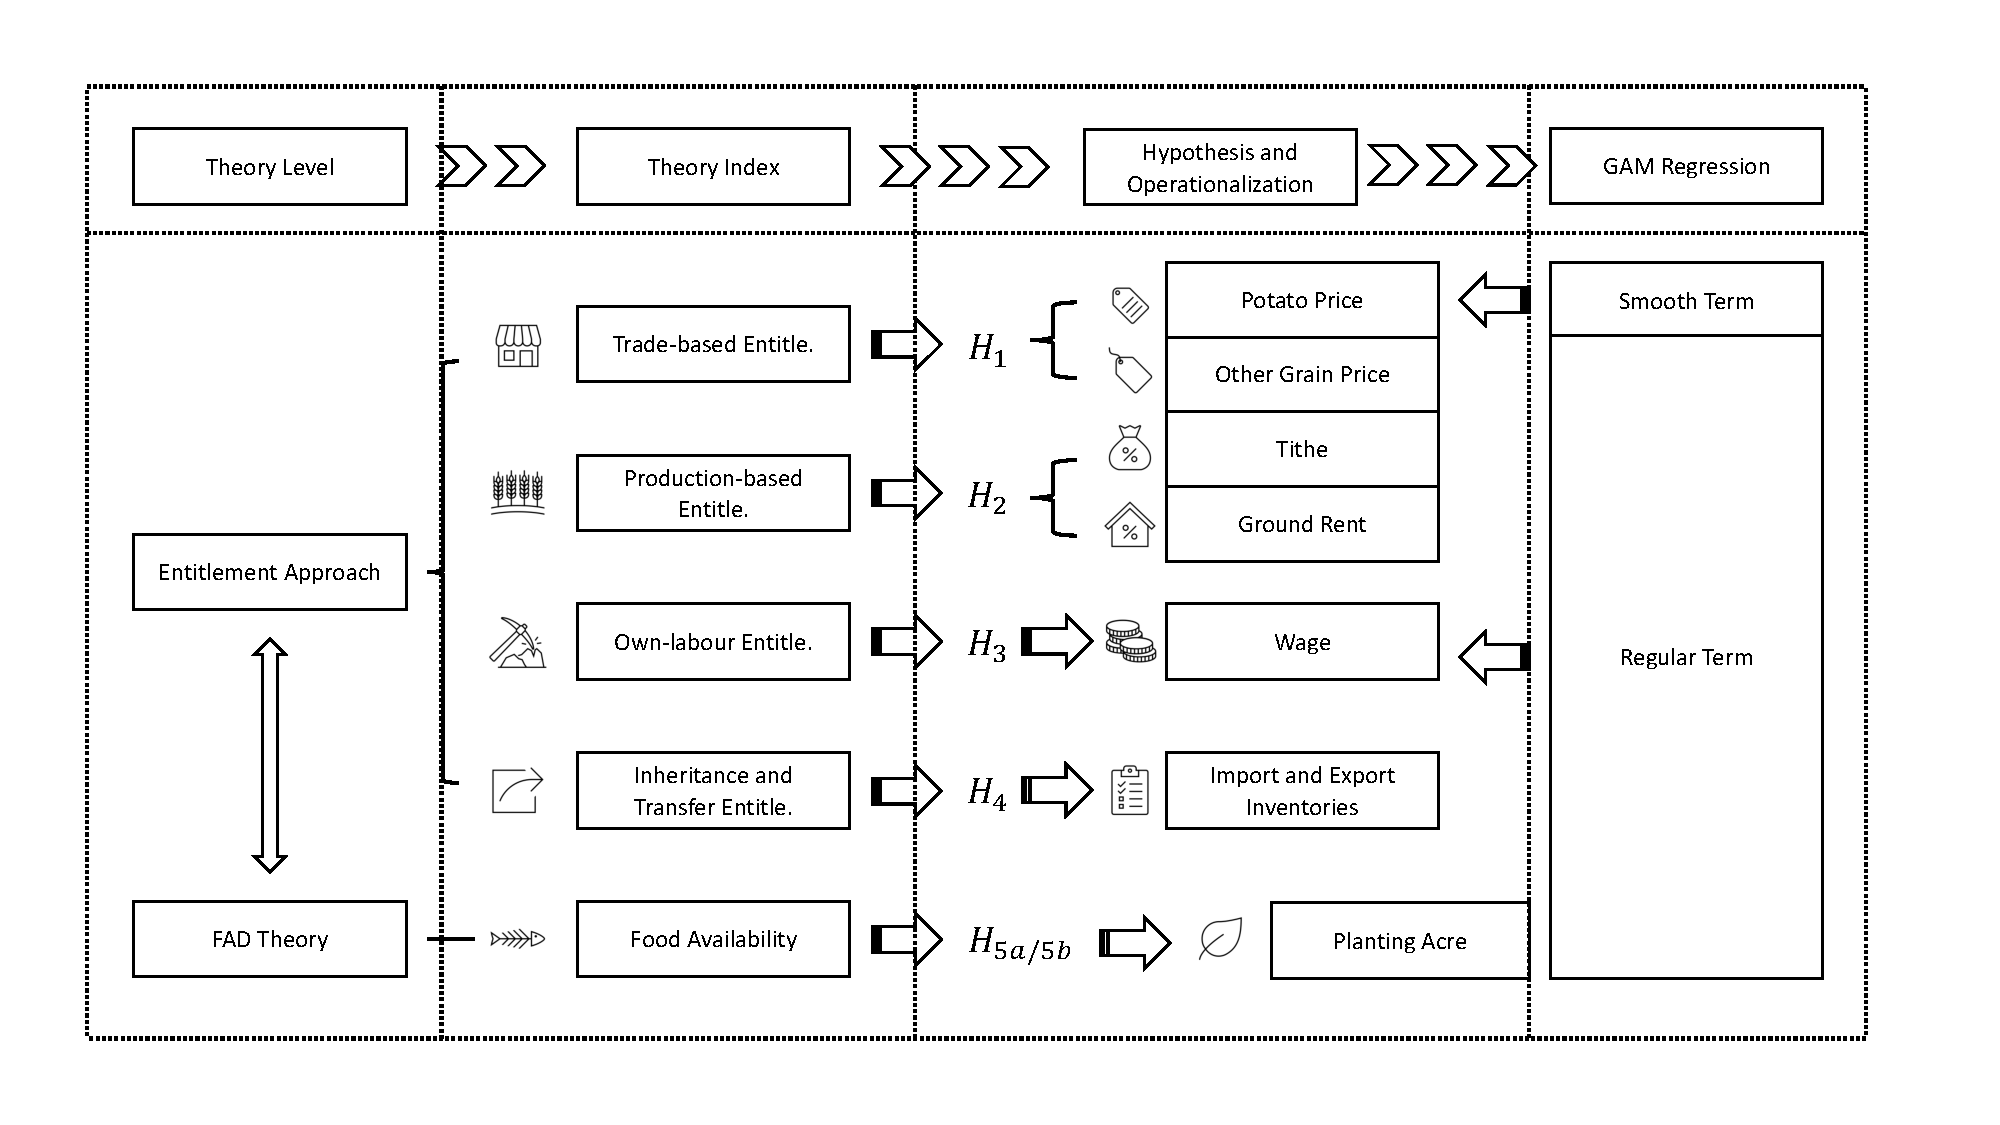
\includegraphics[width=1.5\textheight]{../03_outputs/Framework.pdf}
    \end{figure}
\end{landscape}

\section{Replication}
All the replication file can be found in this website:

\url{https://github.com/chxiii/Dissertation_Summer2024}



